\chapter{Rezultati}
U jednom poglavlju, kako već ide konkretna struktura rada, nakon definiranja
modela uobičajeno se navode rezultati. Bilo da se radi o numeričkim,
eksperimentalnim rezultatima, rezultatima primjene neke analitičke metode ili
rezultatima procesa konstruiranja i sl.

\section{Prikaz rezultata}
Pri prikazu rezultata (npr. slika~\ref{fig:rez}) nužno je obratiti pažnju na
nedvosmisleno označavanje, 
kako veličina koje se prikazuju tako i njenih jedinica (koje bi trebale biti u
skladu sa SI sustavom, u rijetkim slučajevima i po potrebi uz njih moguće je dodati i neke druge
jedinice koje su uvriježene u praksi, kao npr. imperijalne jedinice u
zrakoplovstvu). Isto tako, za slučaj više varijabli i/ili u više varijanti
potrebno je sve označiti na samoj slici ili u njenom zaglavlju.
\begin{figure}
  \centering
  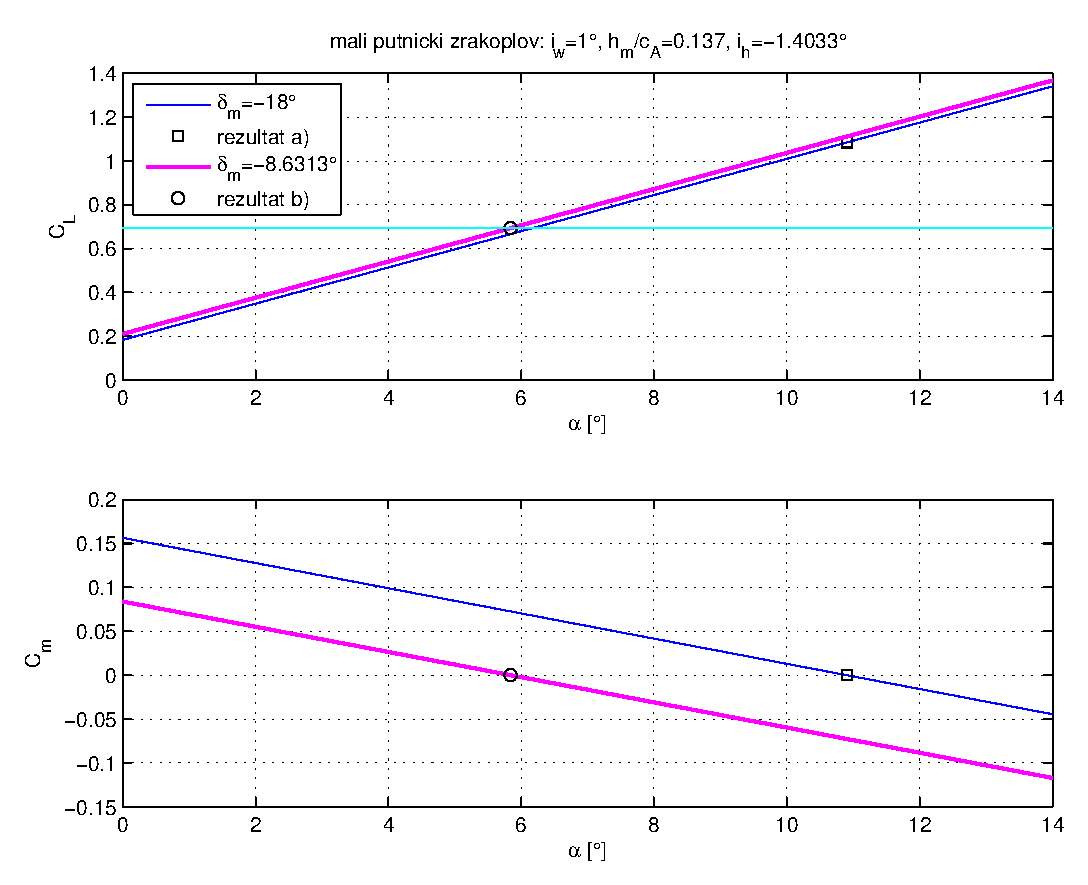
\includegraphics[width=0.95\textwidth]{rezultat}\\
  \hangcaption{Primjer prikaza rezultat: ako neka oznaka/krivulja/podatak sa
  slike nije opisan na samoj slici može ga se opisati u ovom zaglavlju;
  napomena: $C_L$ i $C_m$ su bezdimenzionalne veličine}
  \label{fig:rez}
\end{figure}

